\documentclass[10pt]{article}
\usepackage[polish]{babel}
\usepackage[utf8]{inputenc}
\usepackage[T1]{fontenc}
\usepackage{amsmath}
\usepackage{amsfonts}
\usepackage{amssymb}
\usepackage[version=4]{mhchem}
\usepackage{stmaryrd}
\usepackage{graphicx}
\usepackage[export]{adjustbox}
\graphicspath{ {./images/} }

\title{LIGA MATEMATYCZNA im. Zdzisława Matuskiego GRUDZIEŃ 2015 SZKOŁA PODSTAWOWA }

\author{}
\date{}


\begin{document}
\maketitle
\section*{ZADANIE 1.}
Do zapakowania jest więcej niż 150 bombek, ale mniej niż 200. Mamy dwa rodzaje opakowań do wyboru. Gdy włożymy do pudełek po 10 sztuk, to zostaną 4 bombki, a gdy zapakujemy po 8 sztuk, to też zostaną 4. Ile bombek jest do zapakowania? Ile należy wziąć pudełek każdego rodzaju, aby je zapełnić i aby wszystkie bombki były zapakowane? Podaj wszystkie możliwości.

\section*{ZADANIE 2.}
Wykaż, że liczba \(10^{49}+20\) jest podzielna przez 12 .

\section*{ZADANIE 3.}
Pan Jan hoduje koty. Ma ich tyle, że gdy dodał liczbę kocich ogonów, uszu i łapek, to otrzymał ponad 100. Gdy zsumował tylko liczbę ogonów i łap, otrzymał mniej niż 80. Ile kotów ma pan Jan?

\section*{ZADANIE 4.}
Czarodziej podarował Ani zaczarowaną szkatułkę i podał dwa zaklęcia. Szkatułka ta na jedno z zaklęć powiększa swoją zawartość o jednego denara, a na drugie podwaja liczbę denarów znajdujących się w niej. Podaj najmniejszą liczbę zaklęć, jakie trzeba wypowiedzieć, aby w szkatułce (na początku pustej) znalazło się 40 denarów (nie wyjmujemy monet ze szkatułki).

\section*{ZADANIE 5.}
Z ilu najmniejszych kwadracików (dwa z nich zaznaczono na czarno) składa się duży kwadrat o czarnym obwodzie?\\
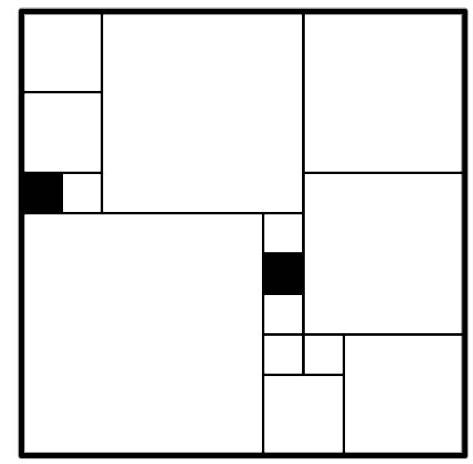
\includegraphics[max width=\textwidth, center]{2024_11_21_c1950e5afa96ea9dff65g-1}


\end{document}